%% Riassunto della tesi di laurea magistrale di Dylan Magliano
%% Compilare con: pdflatex -interaction=nonstopmode riassunto_tesi.tex (due passate)
\documentclass[11pt,a4paper]{article}
\usepackage[utf8]{inputenc}
\usepackage[T1]{fontenc}
\usepackage{lmodern}
\usepackage[italian]{babel}
\usepackage[a4paper,top=2.4cm,bottom=2.4cm,left=2.5cm,right=2.5cm]{geometry}
\usepackage{microtype}
\usepackage{amsmath,amssymb}
\usepackage{graphicx}
\usepackage{booktabs}
\usepackage{array}
\usepackage{enumitem}
\usepackage{xcolor}
\usepackage[most]{tcolorbox}
\usepackage{caption}
\usepackage{titlesec}
\usepackage{fancyhdr}
\usepackage{lastpage}
\usepackage{float}
\usepackage[hidelinks]{hyperref}
\hypersetup{pdftitle={Riassunto della tesi - Dylan Magliano},pdfauthor={Dylan Magliano},pdfsubject={Dai pixel ai portafogli finanziari: generare scenari di mercato realistici tramite variational autoencoder}}

\definecolor{polito}{RGB}{0,51,102}
\definecolor{accent}{RGB}{127,63,0}
\definecolor{grigio}{RGB}{95,95,95}

\titleformat{\section}{\Large\bfseries\color{polito}}{\thesection}{0.7em}{}
\titlespacing*{\section}{0pt}{1.6ex plus 0.6ex minus 0.3ex}{1.0ex plus 0.3ex}
\titleformat{\subsection}{\large\bfseries\color{polito!85!black}}{\thesubsection}{0.6em}{}
\titlespacing*{\subsection}{0pt}{1.2ex plus 0.4ex minus 0.2ex}{0.6ex plus 0.2ex}
\titleformat{\paragraph}[runin]{\bfseries}{}{0em}{}
\titlespacing*{\paragraph}{0pt}{0.8ex plus 0.3ex}{0.6em}

\newtcolorbox{riquadro}[2][]{%
  enhanced, breakable,
  colback=polito!4, colframe=polito, boxrule=0.6pt, arc=2pt,
  fonttitle=\bfseries, coltitle=white, colbacktitle=polito,
  title={#2}, left=6pt, right=6pt, top=5pt, bottom=5pt,
  before skip=8pt plus 2pt, after skip=8pt plus 2pt, #1}

\captionsetup{font=small,labelfont={bf,color=polito},width=0.92\linewidth}
\setlist{nosep, leftmargin=1.4em, itemsep=1.5pt}
\setlength{\parskip}{3pt plus 1pt}
\setlength{\parindent}{0pt}
\renewcommand{\arraystretch}{1.12}
\graphicspath{{./}}
\renewcommand{\floatpagefraction}{0.8}
\renewcommand{\topfraction}{0.85}
\renewcommand{\bottomfraction}{0.6}
\renewcommand{\textfraction}{0.1}

\pagestyle{fancy}
\fancyhf{}
\fancyhead[L]{\small\color{grigio}Riassunto della tesi -- Dylan Magliano}
\fancyhead[R]{\small\color{grigio}Politecnico di Torino, A.A. 2025-2026}
\fancyfoot[C]{\small\color{grigio}\thepage\ / \pageref{LastPage}}
\renewcommand{\headrulewidth}{0.3pt}
\renewcommand{\headrule}{\hbox to\headwidth{\color{polito!60}\leaders\hrule height \headrulewidth\hfill}}

\hyphenation{auto-en-co-der va-ria-tio-nal Cho-le-sky Mar-chen-ko Fro-be-nius}

\begin{document}

%% ---------------------------------------------------------------- Testata
\begin{center}
  {\small\color{grigio}\textsc{Politecnico di Torino} \,$\cdot$\, Corso di Laurea Magistrale in Ingegneria Informatica\\
  Orientamento Artificial Intelligence and Data Analytics \,$\cdot$\, Anno Accademico 2025-2026}\\[1.4ex]
  {\LARGE\bfseries\color{polito}Dai pixel ai portafogli finanziari:\\[0.3ex] generare scenari di mercato realistici\\[0.3ex] tramite variational autoencoder\par}
  \vspace{1.2ex}
  {\large Riassunto della tesi di laurea magistrale\par}
  \vspace{1.4ex}
  \begin{tabular}{@{}r@{\hspace{0.8em}}l@{}}
    \textcolor{grigio}{Candidato} & Dylan Magliano (matricola s337915)\\
    \textcolor{grigio}{Relatore} & prof. Flavio Giobergia, Politecnico di Torino\\
    \textcolor{grigio}{Correlatori} & dott. Sergio Caprioli e dott. Emanuele Cagliero, Intesa Sanpaolo\\
  \end{tabular}
  \vspace{0.8ex}
  {\color{polito!60}\rule{0.6\linewidth}{0.4pt}}
\end{center}

{\small\color{grigio}Questo documento riassume la tesi (tre parti, nove capitoli) seguendone l'ordine. Le figure e le tabelle sono riprese o ricavate dalla tesi; i riferimenti tra parentesi rimandano ai suoi capitoli e sezioni.\par}

%% ---- sezione A: in-breve+problema ----
\begin{riquadro}{La tesi in un paragrafo}
Il lavoro, svolto in collaborazione con Intesa Sanpaolo, affronta i limiti delle matrici di correlazione empiriche, affette da rumore statistico e vincolate all'unica traiettoria offerta dalla storia. A partire dai rendimenti giornalieri di 362 titoli dell'S\&P 500 con quotazioni ininterrotte nel periodo 2000--2020, la tesi segue un percorso incrementale, dal benchmark lineare con la PCA all'autoencoder lineare (AE lineare), all'autoencoder profondo (AE) e infine al variational autoencoder (VAE). Ogni modello è addestrato non sulla matrice grezza ma sul vettore del fattore di Cholesky, così che la ricomposizione $L L^{\top}$ garantisca per costruzione la semidefinita positività. L'obiettivo è generare scenari sintetici delle matrici di correlazione a un orizzonte nominale di 21 giorni lavorativi, costruiti ricampionando transizioni storiche dello spazio latente del VAE, per stimare la possibile variabilità delle correlazioni a quell'orizzonte in ottica di rischiosità. Il ricampionamento è un block-bootstrap degli incrementi latenti giornalieri, ancorato allo stato di mercato osservato all'ultima data del campione, in luogo del campionamento dal prior. Nella verifica aggregata tutti i 1000 scenari risultano conformi ai cinque fatti stilizzati delle matrici di correlazione finanziarie e definiti positivi (autovalore minimo fra 0.0101 e 0.0185), in linea con la semidefinita positività garantita per costruzione.
\end{riquadro}

\section{Il problema e l'obiettivo}

\paragraph{Correlazione e diversificazione.} Nella Modern Portfolio Theory di Markowitz (1952) il rischio di un portafoglio dipende soprattutto dal co-movimento dei titoli, catturato dalla matrice di correlazione: con correlazioni inferiori a 1 il rischio complessivo è strettamente inferiore alla somma dei rischi individuali (cap.~2, \S2.1). Basarsi sulla sola matrice storica significa però assumere interdipendenze immutate, mentre la struttura delle correlazioni è soggetta a continui cambiamenti, specie nei periodi di stress.

\paragraph{Tre limiti della matrice empirica.} Le criticità sono di tre ordini:
\begin{itemize}
\item la stima è rumorosa: l'accuratezza dello stimatore dipende dal parametro di spettro $q = N/T$ e, quando il numero di asset $N$ è confrontabile con la lunghezza $T$ della serie, la Random Matrix Theory (Bouchaud e Potters, 2011; Plerou et al., 2002) descrive la comparsa di autovalori artificialmente piccoli e grandi (\S2.2);
\item la storia offre una sola traiettoria e preclude configurazioni alternative o eventi estremi plausibili ma mai verificatisi nel campione (\S1.1);
\item i motori Monte Carlo classici del risk management usano un'unica matrice fissa lungo l'orizzonte: la dipendenza non può cambiare regime né rappresentare l'aumento brusco delle correlazioni nei ribassi (Longin e Solnik, 2001; Ang e Chen, 2002; \S2.3).
\end{itemize}

\paragraph{L'obiettivo.} Data la natura intrinsecamente stocastica dei mercati, la tesi giudica eccessivamente ambiziosa la previsione puntuale della matrice futura: l'obiettivo realistico è approssimare con insiemi di scenari la distribuzione delle configurazioni possibili. Il lavoro si propone quindi, come anticipato nel riquadro iniziale, di generare scenari sintetici delle matrici di correlazione a un orizzonte nominale di 21 giorni lavorativi (circa un mese), costruiti ricampionando transizioni storiche dello spazio latente, per stimare la possibile variabilità delle correlazioni a quell'orizzonte in ottica di rischiosità (\S2.1; \S8.1).

\paragraph{Perché i modelli generativi profondi.} Rispetto ai metodi tradizionali, che tendono a linearizzare le relazioni o a restare vincolati alla dinamica storica, i VAE (Kingma e Welling, 2013) mappano le matrici in uno spazio latente continuo da cui campionare stocasticamente. I ``pixel'' del titolo alludono alla filiazione di questi modelli dal dominio delle immagini: le matrici sono trattate come oggetti strutturati ad alta dimensionalità, pur con il fattore di Cholesky vettorizzato come input. I precedenti sono CorrGAN (Marti, 2020), che campiona matrici di correlazione con una GAN e ne verifica l'output sui cinque fatti stilizzati, e il lavoro di riferimento di Caprioli et al. (2024). Quest'ultimo addestra un VAE su matrici storiche e ne ricampiona le coordinate latenti, in analogia con la procedura del cap.~8 (\S1.2).

\paragraph{Il ruolo di Cholesky.} Ogni matrice di correlazione valida è per definizione semidefinita positiva (PSD, autovalori non negativi); la decomposizione di Cholesky richiede la condizione più forte di definita positività (rango pieno) e fornisce una matrice triangolare inferiore $L$ con $C = L L^{\top}$, usata per correlare vettori gaussiani $\mathbf{z} \sim \mathcal{N}(0, I_N)$ (\S2.3). Poiché l'output di un modello generativo non è garantito PSD, i modelli lavorano sul fattore $L$, la cui ricomposizione $L L^{\top}$ assicura la semidefinita positività per costruzione.

\paragraph{Obiettivi specifici e limiti dichiarati.} Gli obiettivi specifici (\S1.3) sono tre: una pipeline di pre-processing sull'S\&P 500 (2000--2020) con parametrizzazione di Cholesky; uno studio comparativo del potere ricostruttivo lungo il percorso PCA, AE lineare, AE profondo, con metriche di errore e topologiche al variare di $K$; l'integrazione probabilistica tramite VAE, campionando matrici inedite e verificandone la conformità ai cinque fatti stilizzati. Un limite è dichiarato fin dall'inizio: il filtro di continuità delle quotazioni introduce un survivorship bias (esclusione delle aziende fallite o uscite dall'indice), accettato per disporre di un panel bilanciato senza dati mancanti. Resta fuori perimetro la traduzione degli scenari in misure di rischio di portafoglio, indicata come primo sviluppo futuro (\S9.3).

%% ---- sezione B: fatti-stilizzati ----
\section{La matrice di correlazione e i cinque fatti stilizzati}

La matrice di correlazione empirica nasce dai log-rendimenti giornalieri $r_{i,t} = \ln(P_{i,t}/P_{i,t-1})$, preferiti ai prezzi perché stazionari, sui quali si stima la correlazione di Pearson fra coppie di titoli (\S5.2). Essa è simmetrica, a diagonale unitaria, con coefficienti in $[-1, 1]$ e semidefinita positiva (PSD); con finestre di stima lunghe il doppio del numero di titoli (nella tesi $T_w = 2N$) è anche definita positiva, condizione più forte richiesta dalla decomposizione di Cholesky (\S2.3, \S5.2). La validità formale, però, non significa realismo: anche la matrice di correlazione di serie di puro rumore soddisfa questi vincoli. Per giudicare il realismo il capitolo 3 ricorre a cinque fatti stilizzati --- regolarità empiriche persistenti nel senso di Cont (2001) --- già impiegati come protocollo di validazione da Marti (2020) per CorrGAN e da Caprioli et al.\ (2024) per un VAE. Le proprietà sono illustrate sulla matrice di esempio n.~100 ($N = 362$, finestra di 724 giorni).

\begin{itemize}[leftmargin=*, itemsep=2pt]
\item \textbf{Distribuzione pairwise spostata verso valori positivi.} Sotto indipendenza i coefficienti sarebbero centrati sullo zero; nei mercati reali la media è positiva, tipicamente in $[0.2, 0.5]$, per l'effetto mercato. Matrice n.~100: media 0.2334, mediana 0.2257.
\item \textbf{Spettro oltre la banda di Marchenko-Pastur.} Per dati i.i.d.\ nel limite $N, T \to \infty$ con $q = N/T$ fissato, gli autovalori restano nel bulk $[\lambda_-, \lambda_+]$, $\lambda_\pm = (1 \pm \sqrt{q})^2$, e per $q = 0.5$ vale $\lambda_+ = 2.914$. La matrice n.~100 ne ha 9 sopra la soglia: $\lambda_1 = 88.753$, pari al 24.5\% della varianza totale (market mode), e altri otto letti come modi settoriali.
\item \textbf{Proprietà di Perron-Frobenius empirica.} $\lambda_1$ ha molteplicità uno e le componenti dell'autovettore $\mathbf{v}_1$ hanno tutte lo stesso segno. Il teorema fornisce solo una condizione sufficiente (elementi non negativi) che le matrici reali non soddisfano: l'uniformità di segno è una regolarità da verificare caso per caso. Essa è tanto più notevole perché Hüttner e Mai (2019) dimostrano che la possiede solo una frazione $2^{1-d}$ delle matrici di correlazione di dimensione $d$. Una minoranza delle finestre storiche la viola per un singolo titolo debolmente anticorrelato con il resto del paniere (filtro di \S5.3).
\item \textbf{Struttura gerarchica.} Con la distanza di Mantegna $d_{ij} = \sqrt{2(1 - C_{ij})}$ e un clustering ad average linkage, il dendrogramma mostra blocchi corrispondenti ai settori GICS: sulla matrice n.~100 le fusioni intra-settore avvengono tipicamente sotto 1.0, quelle inter-settore sopra 1.15.
\item \textbf{MST scale-free.} Il Minimum Spanning Tree sulle stesse distanze (Mantegna, 1999) ha una distribuzione di grado a legge di potenza $P(k) \propto k^{-\gamma}$ con $2 < \gamma < 3$ (pochi hub, ampia periferia): sulla matrice n.~100, $\gamma = 2.207$ e grado massimo 14.
\end{itemize}

\paragraph{Il benchmark di rumore (\S3.7).} Per verificare che le proprietà non siano artefatti della dimensionalità campionaria, lo stesso protocollo è applicato a una matrice di controllo ottenuta da $N = 362$ serie di rumore gaussiano i.i.d.\ di lunghezza $T = 724$, le stesse dimensioni della matrice reale. Il controllo non supera nessuna delle cinque verifiche: media pairwise 0.0000 con deviazione standard 0.0373, in accordo con il valore atteso $1/\sqrt{T}$; $\lambda_1 = 2.907$ e nessun autovalore oltre $\lambda_+$; 50.8\% di componenti negative in $\mathbf{v}_1$; nessun blocco nel dendrogramma, con fusioni schiacciate a circa $\sqrt{2}$ e colori settoriali interlacciati; grado massimo dell'MST 6 contro 14 e distribuzione di grado concava, senza legge di potenza.

I cinque fatti sono quindi la firma geometrica che separa l'informazione di mercato dal rumore: è ciò che il modello generativo dovrà riprodurre e che, nel capitolo 8, diventa il protocollo di validazione dei 1000 scenari sintetici. Le ricostruzioni del capitolo 7 sono invece valutate con metriche di errore e di similarità fra MST (\S6.5).

%% ---- sezione C: modelli+dati ----
\section{Dalla PCA al VAE: i modelli}

Il capitolo 4 presenta, in ordine di complessità crescente, i quattro modelli confrontati.

\paragraph{PCA.} È il riferimento lineare: una proiezione ortogonale $\mathbf{z} = W^{\top} \mathbf{x}$, $\hat{\mathbf{x}} = W W^{\top} \mathbf{x}$, ottima in termini di errore quadratico medio, con soluzione analitica negli autovettori dominanti della covarianza. Il limite è strutturale: assume che la manifold dei dati sia un iperpiano lineare, mentre i co-movimenti di mercato (tail dependence, gerarchie settoriali) presentano strutture non lineari.

\paragraph{Autoencoder lineare.} Con attivazioni identità, senza bias né weight decay, l'autoencoder a un solo strato converge, per il risultato di Bourlard e Kamp (1988), al sottospazio delle prime $K$ componenti principali: serve da sanity check e benchmark strutturale di partenza.

\paragraph{Autoencoder profondo.} Strati nascosti non lineari possono catturare la curvatura della manifold, ma lo spazio latente, non vincolato ad alcun prior e organizzato dal solo errore di ricostruzione, risulta irregolare, con ampie zone vuote. Il limite non sta nella qualità della compressione ma nell'obiettivo di addestramento, che non prevede alcun campionamento di nuovi punti nello spazio latente, operazione per la quale il modello non è addestrato (cap.~7); si tratta di una premessa metodologica, non sottoposta a verifica empirica nella tesi.

\paragraph{VAE.} Il Variational Autoencoder (Kingma e Welling, 2013) fa emettere all'encoder una distribuzione $q_\phi(\mathbf{z}|\mathbf{x}) = \mathcal{N}(\boldsymbol{\mu}, \mathrm{diag}(\boldsymbol{\sigma}^2))$, campionata con il reparameterization trick $\mathbf{z} = \boldsymbol{\mu} + \boldsymbol{\sigma} \odot \boldsymbol{\epsilon}$, $\boldsymbol{\epsilon} \sim \mathcal{N}(0, I)$. La loss somma un termine di ricostruzione, che nel cap.~6 è la divergenza di Jeffreys fra matrici di correlazione, e il regolarizzatore $\beta\, D_{\mathrm{KL}}(q_\phi(\mathbf{z}|\mathbf{x})\,\|\,\mathcal{N}(0, I))$ nello spazio latente, con $\beta = 1$. La KL addensa le distribuzioni attorno all'origine e le sovrappone, riducendo le zone vuote dello spazio latente. Rispetto alle GAN di CorrGAN (Marti, 2020), il VAE offre un addestramento tipicamente più stabile, privo del gioco minimax, e uno spazio latente esplicitamente strutturato e ricampionabile, proprietà sfruttata anche da Caprioli et al. (2024) per costruire scenari di rischio interpretabili. Il campionamento dal prior, possibile in linea di principio, è sostituito nella tesi dal block-bootstrap di incrementi storici nello spazio latente (cap.~8), ancorato allo stato di mercato osservato.

\section{Dati e pre-processing}

\paragraph{Dataset.} Il dataset raccoglie i prezzi di chiusura rettificati dei titoli dell'S\&P 500 dal 2000 al 2020, periodo che include fasi espansive, recessive e di stress. Sono mantenuti i soli titoli con quotazioni ininterrotte sull'intero arco, $N = 362$: la tesi dichiara il survivorship bias e legge il campione come ``popolazione condizionata alla sopravvivenza''. La classificazione GICS è stata ricostruita con un modello linguistico (gemini-2.5-flash, few-shot): 360 titoli su 362, con ABC e CERN non classificati.

\paragraph{Finestre mobili.} La correlazione è stimata sui log-rendimenti, stazionari a differenza dei prezzi, su una finestra mobile di $T_w = 724$ giorni con passo $S = 10$. Il valore $T_w = 2N$ fissa per costruzione il rapporto di spettro $q = N/T_w = 0.5$, il regime di Marchenko-Pastur del cap.~3, e assicura che ogni matrice empirica sia di rango pieno, cioè definita positiva, condizione di esistenza e unicità della decomposizione di Cholesky. Dai 5333 log-rendimenti si ottengono 461 matrici.

\paragraph{Filtro di Perron-Frobenius.} Le prime 49 finestre violano l'uniformità di segno del primo autovettore. Sono tutte e sole quelle con osservazioni antecedenti la metà di ottobre 2001 e il solo titolo con componente negativa è sempre NEM (Newmont), unico titolo aurifero del paniere, che durante la bolla dot-com si è mosso da bene rifugio, in controtendenza rispetto al listino. La violazione è dunque riconducibile a un regime eccezionale e circoscritto, non a un artefatto di misura. L'esclusione è dichiarata come scelta di perimetro: il lavoro si limita al regime cooperativo ``standard'', su cui sono definiti i fatti stilizzati del protocollo di validazione, senza pretendere di rappresentare i regimi di disaccoppiamento. Restano 412 matrici.

\paragraph{Ripartizione.} Test preliminari con split cronologico hanno evidenziato un distribution shift: i regimi passati non bastavano a generalizzare sui successivi. La tesi adotta perciò un random shuffle dell'intero bacino, ripartito 70/20/10 in 288, 82 e 42 matrici, così da distribuire omogeneamente fasi volatili e stabili nei tre set. Lo shuffle non elimina però la sovrapposizione fra finestre adiacenti, fino al 98.6\% delle osservazioni (714 giorni su 724): matrici quasi identiche possono finire in set diversi, limite dichiarato.

\paragraph{Parametrizzazione di Cholesky.} Un primo approccio usava il triangolo inferiore stretto della matrice di correlazione ($D = 65\,341$), con clipping in $[-1, 1]$. È stato abbandonato perché non offre alcuna garanzia di semidefinita positività, proprietà globale dello spettro, non imponibile coefficiente per coefficiente: le verifiche spettrali hanno rilevato autovalori negativi, e uno solo basta a far fallire la decomposizione di Cholesky. La parametrizzazione definitiva vettorizza il fattore $L$ di $C = L L^{\top}$, diagonale inclusa, con $D = N(N+1)/2 = 65\,703$. Per qualunque output del decoder, $\hat{L}\hat{L}^{\top}$ è una matrice di Gram, dunque semidefinita positiva per costruzione, a prescindere dalla qualità dell'apprendimento; la rinormalizzazione a diagonale unitaria $\hat{R} = \Delta^{-1/2}\hat{C}\Delta^{-1/2}$, con $\Delta = \mathrm{diag}(\hat{C})$, preserva la semidefinita positività per la legge d'inerzia di Sylvester. Lo stesso vettore $\mathbf{x} \in \mathbb{R}^{65\,703}$ è l'input di tutti e quattro i modelli.

\begin{riquadro}{La pipeline in numeri}
5334 quotazioni giornaliere $\rightarrow$ 5333 log-rendimenti $\rightarrow$ 461 finestre (724 giorni, passo 10) $\rightarrow$ filtro di Perron-Frobenius: $-49$ $\rightarrow$ 412 matrici $\rightarrow$ shuffle 70/20/10 $\rightarrow$ 288 / 82 / 42 $\rightarrow$ fattore di Cholesky vettorizzato, $D = 65\,703$.
\end{riquadro}

%% ---- sezione D: setup+risultati ----
\section{Architetture e setup sperimentale}

\paragraph{Benchmark lineari.} La PCA (\S6.1) è addestrata sul solo Training Set standardizzato con $K \in \{3, 10, 20, 100\}$. L'AE lineare (\S6.2) ha un solo layer denso per encoder e decoder, attivazione identità, senza bias né weight decay, ed è ottimizzato sull'MSE con Adam (lr $10^{-3}$, batch 64, fino a 5000 epoche) così da convergere alla PCA.

\paragraph{Autoencoder profondo.} L'AE profondo (\S6.3) adotta un imbuto $65\,703 \to 2048 \to 1024 \to 512 \to K$ con decoder speculare, LeakyReLU ($\alpha = 0.01$) sugli strati nascosti, proiezione latente e layer di uscita lineari. La Tanh in uscita è disattivata perché la sua saturazione agli estremi $\pm 1$ rischia di annullare il gradiente, e il vincolo a $[-1, 1]$ è demandato al clipping finale.

\paragraph{VAE.} Il VAE (\S6.4) condivide l'imbuto, ma il bottleneck si biforca in due teste $\mu$ e $\log \sigma^2$; il codice è campionato con il reparameterization trick ($\mathbf{z} = \mu + \sigma \odot \epsilon$, $\epsilon \sim \mathcal{N}(0, I)$) e in valutazione si pone $\mathbf{z} = \mu$. La loss è $\mathcal{L} = \mathcal{L}_{\text{Recon}} + \beta\,\mathcal{L}_{\text{KL}}$ con $\beta = 1$, poiché entrambi gli addendi sono costruiti da divergenze di Kullback-Leibler e sono dunque grandezze omogenee. Il termine $\mathcal{L}_{\text{Recon}}$ è la divergenza di Jeffreys fra $\mathcal{N}(0, R_{\text{orig}})$ e $\mathcal{N}(0, R_{\text{recon}})$, calcolata nel dominio delle correlazioni dopo la ricomposizione di Cholesky nel grafo differenziabile:
\[
\mathcal{L}_{\text{Recon}} = \tfrac{1}{2}\big[\operatorname{Tr}(R_{\text{recon}}^{-1} R_{\text{orig}}) + \operatorname{Tr}(R_{\text{orig}}^{-1} R_{\text{recon}}) - 2N\big].
\]
Le inverse pesano l'errore in termini relativi su tutto lo spettro, dove l'MSE è cieco agli autovalori più piccoli, e la simmetrizzazione equipara sovrastima e sottostima.

\paragraph{Protocollo e metriche.} Il VAE segue il protocollo della Tabella~6.1 (1000 epoche, batch 64, Adam con lr $10^{-3}$ e weight decay $10^{-5}$, Cosine Annealing, seme 42); l'AE profondo adotta lo stesso schema (tipicamente 1000 epoche, Adam, Cosine Annealing, batch 64; \S6.3). Per entrambi il checkpoint conserva i pesi al minimo assoluto della Validation Loss (\S6.5). Oltre a MSE, MAE e norma di Frobenius, la valutazione impiega cinque metriche topologiche sul Minimum Spanning Tree: edge overlap, indice di Jaccard, scarto della average path length pesata e non pesata, sovrapposizione dei nodi a più alta betweenness.

\section{Risultati: compressione e ricostruzione storica}

\paragraph{Convergenza dei modelli lineari.} In linea con il teorema di Bourlard e Kamp (1988), sul Training Set l'AE lineare converge verso l'MSE della PCA a parità di $K$ (scarto relativo inferiore al 20\%; \S7.1). Sul Test Set i due lineari restano molto vicini, con un vantaggio marginale e sistematico della PCA sulle metriche di errore (\S7.2.1) e valori di fatto sovrapponibili su quelle topologiche (\S7.2.2).

\paragraph{Il vantaggio della non linearità.} L'AE profondo supera nettamente i lineari a ogni $K$, senza segni di overfitting: a $K = 20$ l'MSE di test è $0.72 \times 10^{-4}$ contro $2.73 \times 10^{-4}$ della PCA, con lo stesso ordinamento su MAE e norma di Frobenius (\S7.2.1). Il divario si chiude al crescere di $K$ (Frobenius 20.88 contro 4.22 a $K = 3$, 2.85 contro 2.75 a $K = 100$): è un vantaggio di efficienza rappresentativa, poiché l'AE a $K = 10$ raggiunge la qualità della PCA a $K = 100$ (MAE $0.55 \times 10^{-2}$ per entrambi). La curva dell'AE ha un gomito fra $K = 10$ e $K = 20$ (MSE da $0.84$ a $0.72 \times 10^{-4}$, poi $0.73 \times 10^{-4}$ a $K = 100$), da cui $K = 20$ come compromesso metodologico per il VAE.

\paragraph{Metriche topologiche.} Sull'MST lo stesso ordinamento si ripresenta in forma più netta (\S7.2.2). A $K = 3$ i lineari subiscono un crollo topologico: la PCA conserva il 53.7\% degli archi (Jaccard 37.4\%) contro l'87.7\% (78.5\%) dell'AE; a $K = 100$ i tre modelli deterministici convergono sul 90--91\%, che appare un tetto strutturale. Il VAE a $K = 20$ è intermedio su tutte e cinque le metriche, più vicino all'AE (edge overlap 88.4\% contro 83.0\% della PCA e 91.1\% dell'AE), con la cautela dovuta alle metriche più rumorose (Tabella~\ref{tab:k20}, Figura~\ref{fig:mse_mst}).

\begin{table}[htbp]
\centering\small
\begin{tabular}{lccc}
\toprule
Modello & MSE ($\times 10^{-4}$) & MAE ($\times 10^{-2}$) & Edge overlap MST (\%) \\
\midrule
PCA & 2.73 & 1.18 & 83.0 \\
AE lineare & 3.38 & 1.33 & 83.1 \\
AE profondo & 0.72 & 0.51 & 91.1 \\
VAE & 1.55 & 0.86 & 88.4 \\
\bottomrule
\end{tabular}
\caption{Confronto dei quattro modelli a $K = 20$ sul Test Set (dominio Cholesky): errore di ricostruzione (MSE, MAE) e percentuale di archi dell'MST conservati. I valori sono medie sulle 42 matrici del Test Set, tratti dalle Tabelle 7.1 e 7.2 della tesi.}
\label{tab:k20}
\end{table}

\begin{figure}[htbp]
\centering
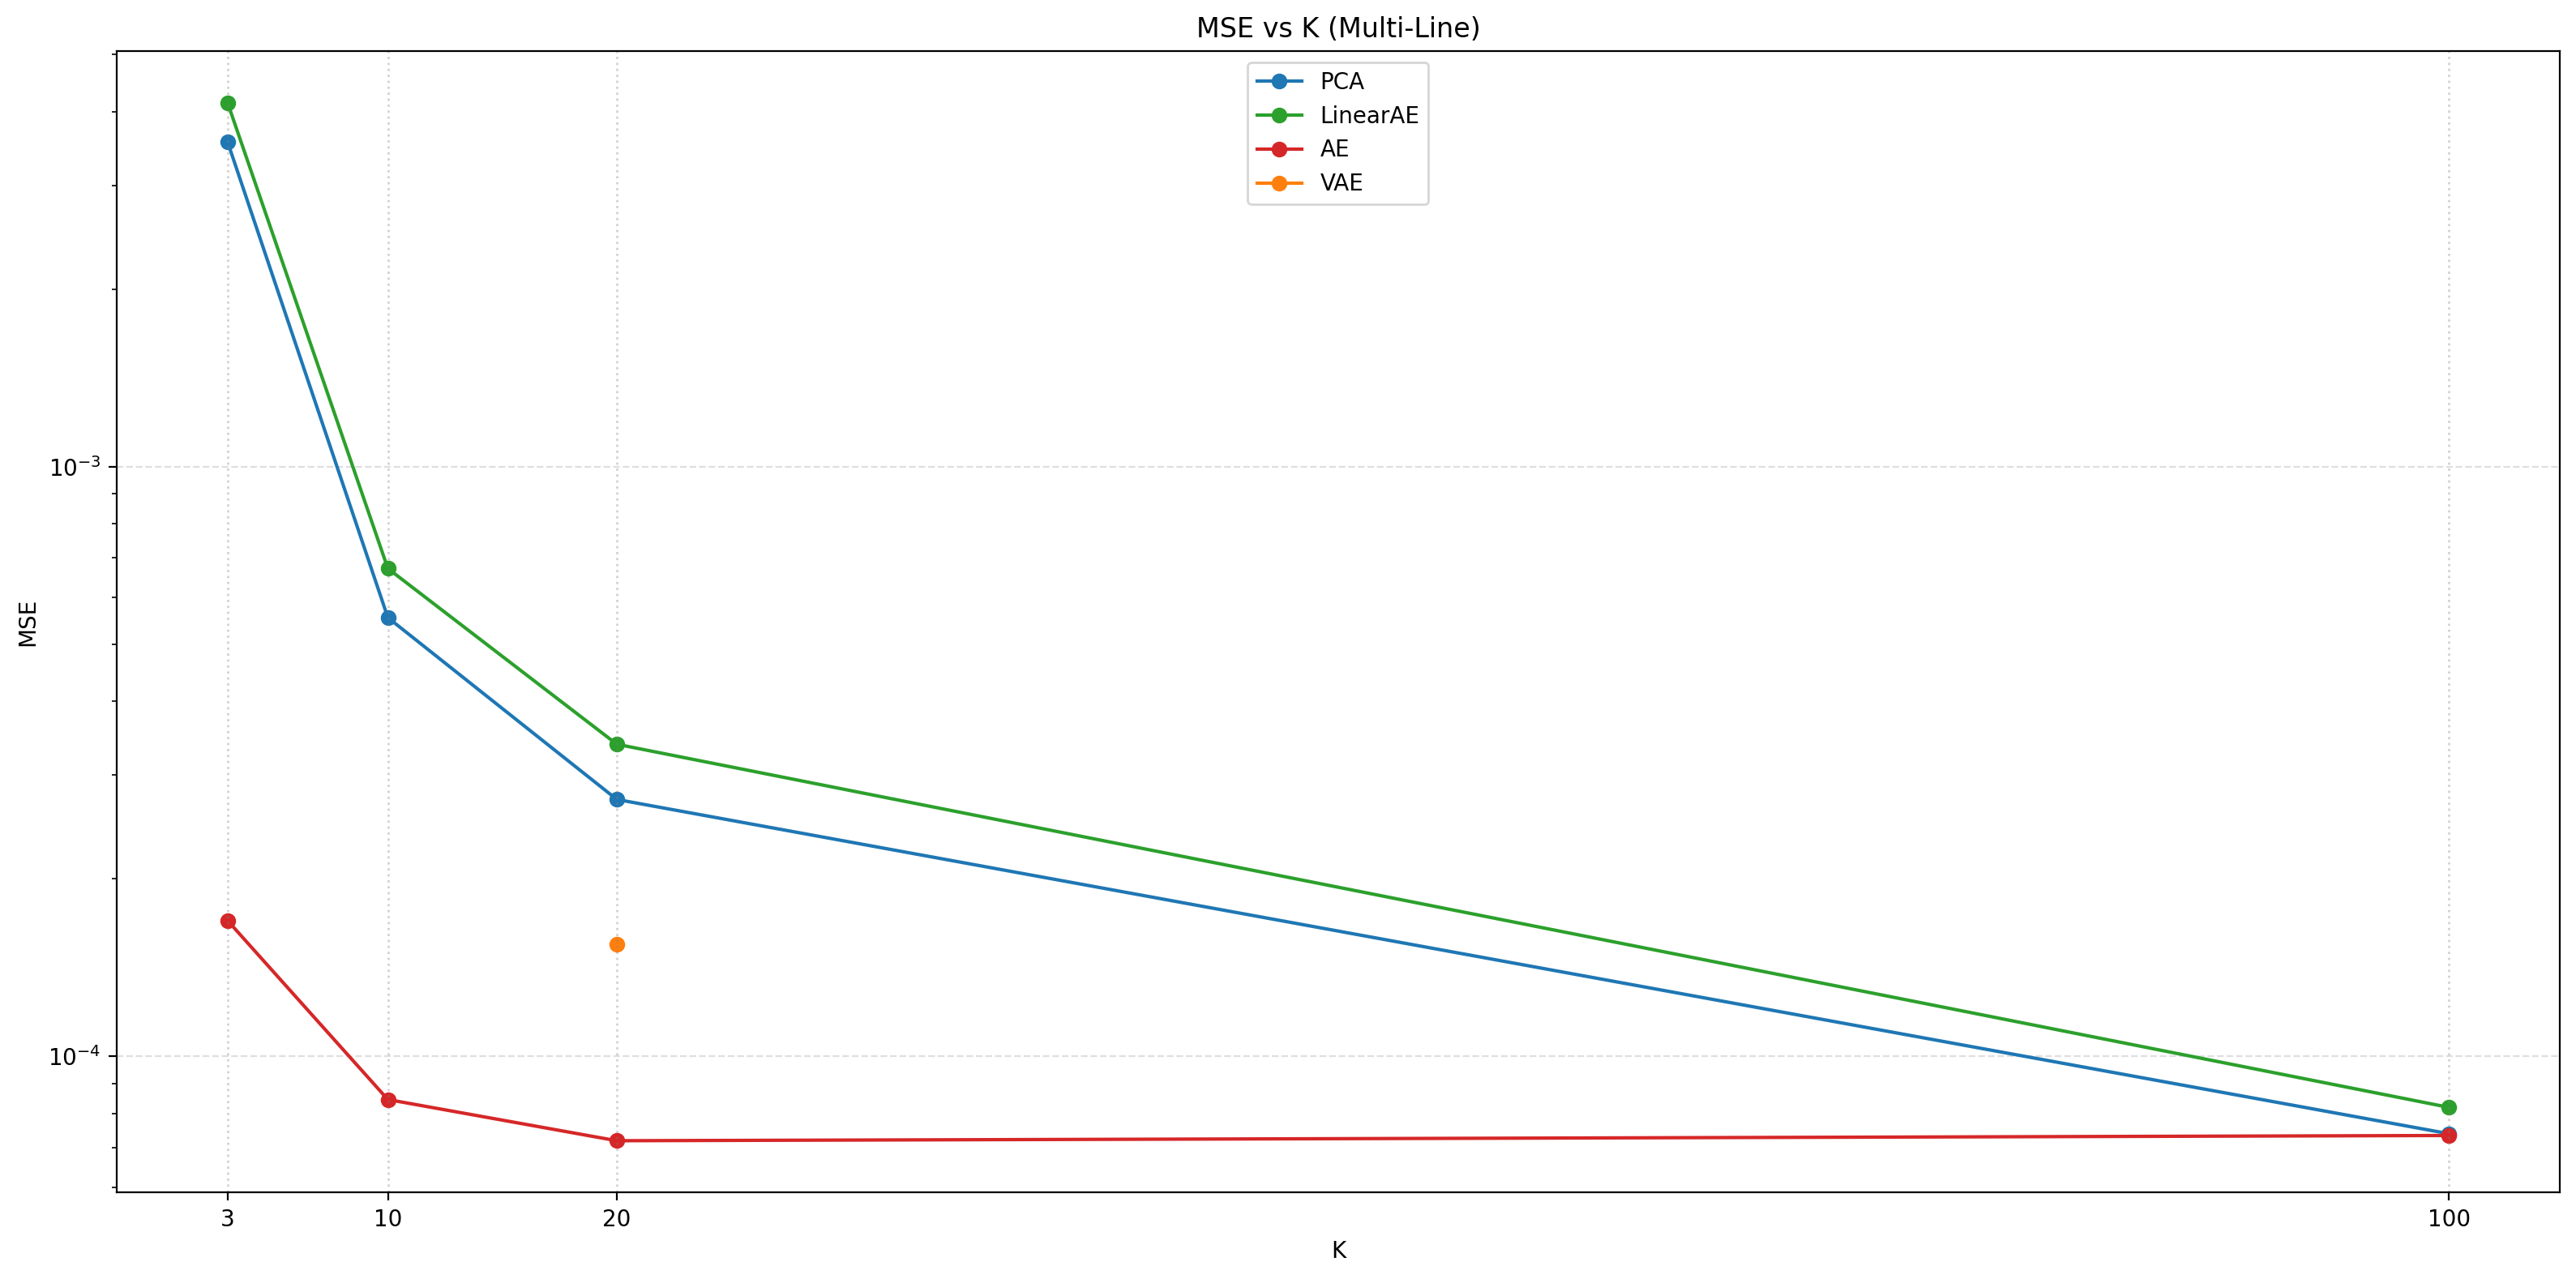
\includegraphics[width=0.84\linewidth]{Pictures/capitolo7/fig_mse_vs_k.png}\par\vspace{5pt}
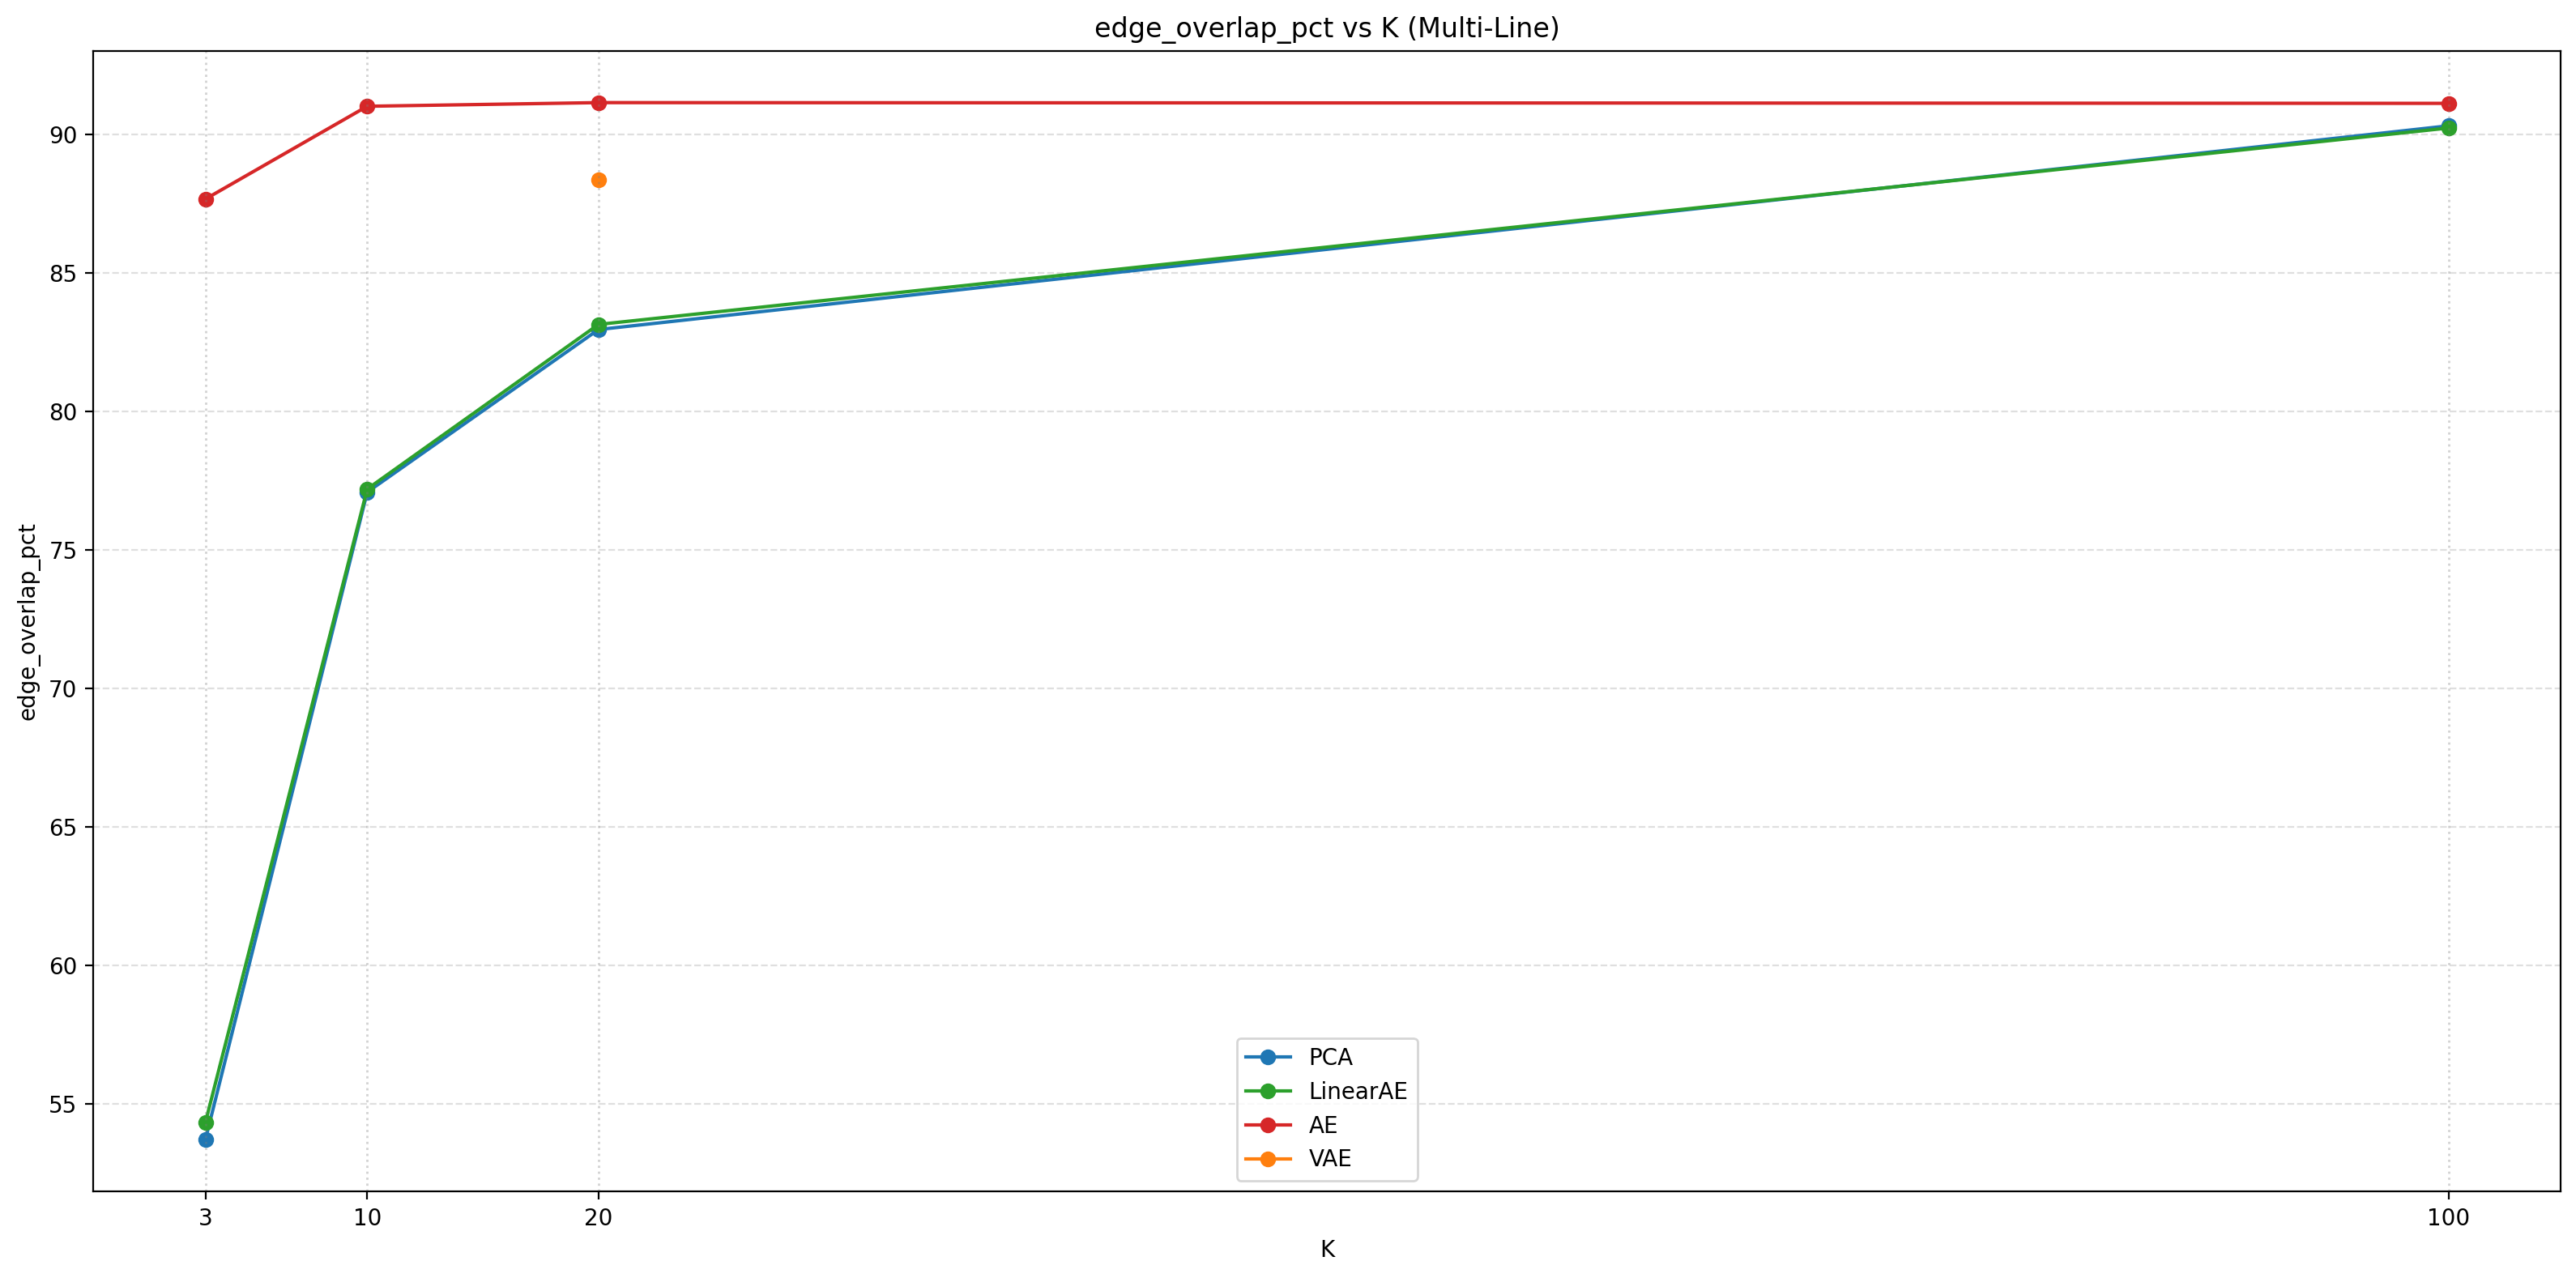
\includegraphics[width=0.84\linewidth]{Pictures/capitolo7/fig_mst_edge_overlap_vs_k.png}
\caption{Errore di ricostruzione MSE (in alto) e percentuale di archi dell'MST conservati (in basso) sul Test Set al variare di $K$ per PCA, AE lineare, AE profondo e VAE (quest'ultimo solo a $K = 20$).}
\label{fig:mse_mst}
\end{figure}

\paragraph{Il VAE al variare di $K$.} Le run a $K = 10$, 20 e 30, identiche salvo $K$ (Tabella~7.3), mostrano un MSE che peggiora con $K$ (da $1.26 \times 10^{-4}$ a $1.88 \times 10^{-4}$), comportamento opposto agli altri modelli, coerente con la competizione fra ricostruzione e termine KL. Le metriche topologiche sono di fatto invarianti (edge overlap 88.6, 88.4 e 88.2\%) e le dimensioni attive con varianza $\geq 0.5$ sono sei in tutte le run: la dimensionalità effettiva appare una proprietà dei dati e la scelta di $K$ poco critica.

\paragraph{Addestramento e spazio latente.} Training e Validation Loss restano allineate fino a circa l'epoca 600. La divergenza di Jeffreys si assesta su un plateau di 7--8 e la KL scende da circa 10 a circa 8, senza divergere né tendere a zero, coerentemente con l'assenza di un collasso globale (\S7.2.4). Lo spettro di varianza dei codici $\mathbf{z} = \mu$ (Figura~\ref{fig:latent}) mostra circa sei dimensioni fortemente attive ($Z_{18}$, $Z_9$, $Z_7$, $Z_1$, $Z_4$, $Z_5$), tre intermedie ($Z_6$, $Z_{10}$, $Z_{12}$) e le restanti in posterior collapse. Le quattro più attive tracciano una manifold continua in cui Training, Validation e Test Set si sovrappongono. Il sottospazio effettivo ha 6--9 dimensioni e quelle in eccesso tendono a collassare, il che offre una chiave di lettura del fatto che l'errore del VAE non decresca con $K$ (\S7.3.1).

\begin{figure}[htbp]
\centering
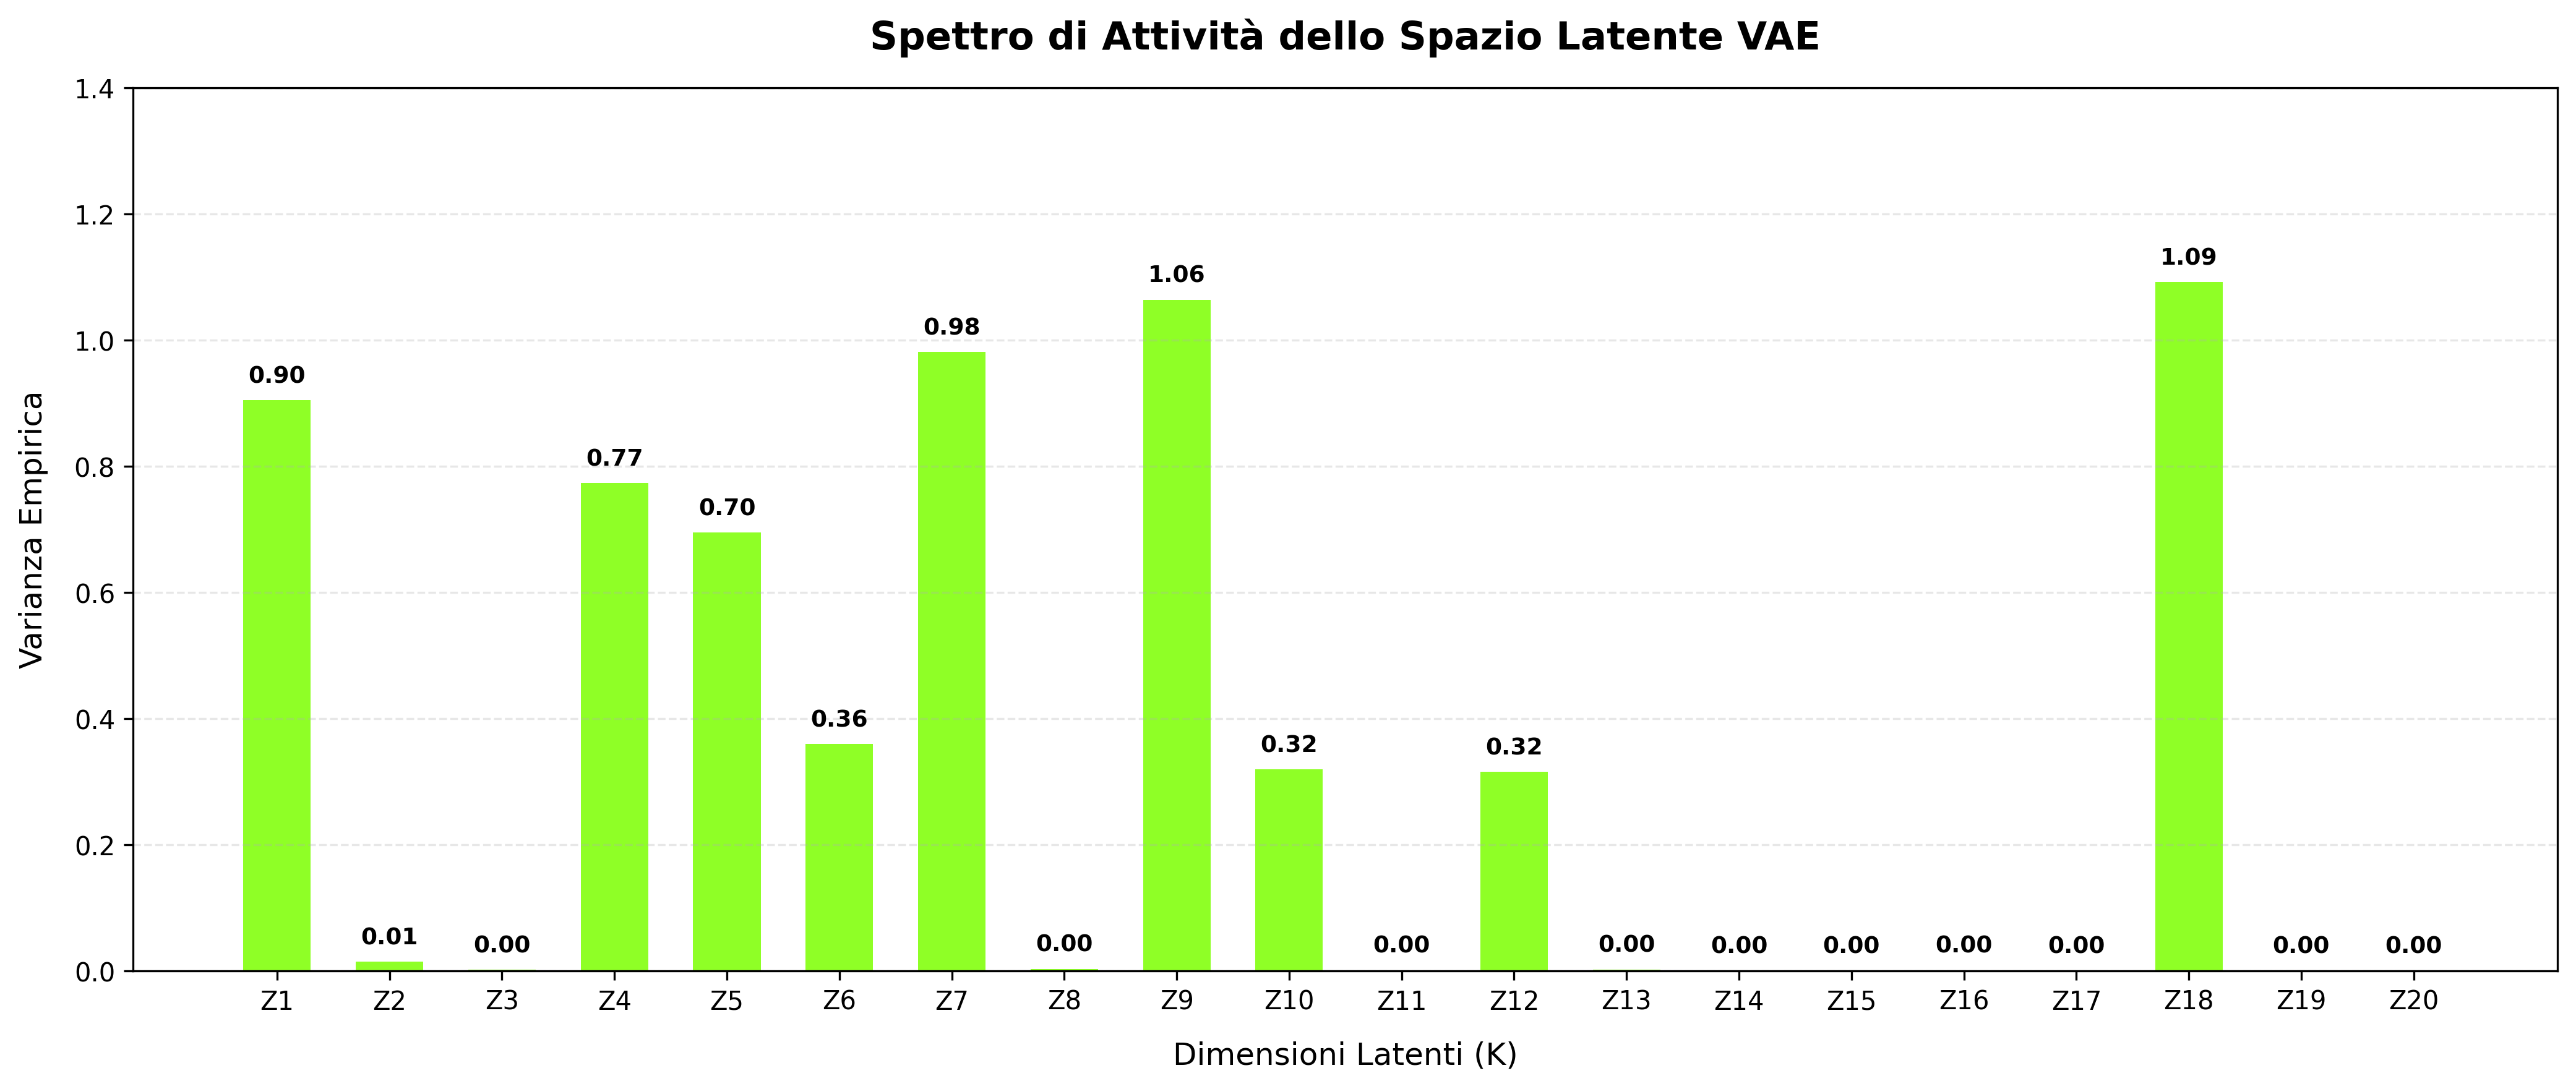
\includegraphics[width=0.9\linewidth]{Pictures/capitolo7/fig_vae_latent_variance_spectrum.png}
\caption{Varianza empirica dei codici latenti $\mathbf{z} = \mu$ delle 288 matrici di training per ciascuna delle 20 dimensioni del VAE definitivo.}
\label{fig:latent}
\end{figure}

\paragraph{Il trade-off.} Il VAE è lievemente meno accurato dell'AE profondo ma superiore ai lineari anche in pura ricostruzione (\S7.3). Il limite dell'AE deterministico, già richiamato, non sta nella qualità della compressione ma in un obiettivo di addestramento che non prevede il campionamento di nuovi punti latenti (premessa metodologica, non esito verificato sperimentalmente). In cambio di uno scarto contenuto, la regolarizzazione variazionale del VAE modella uno spazio latente continuo e denso in cui campionare: per questo è il modello scelto per generare gli scenari.

%% ---- sezione E: generazione ----
\section{Generazione di scenari sintetici e validazione}

\paragraph{Dal prior al block-bootstrap storico (\S8.1).}
La regolarizzazione di Kullback-Leibler permette in linea di principio di generare nuove matrici decodificando $\mathbf{z} \sim \mathcal{N}(0, I)$ campionato dal prior. L'obiettivo della tesi non è però uno scenario plausibile qualsiasi, bensì una distribuzione di scenari sintetici della struttura di correlazione a orizzonte nominale di 21 giorni lavorativi, costruiti ricampionando transizioni storiche dello spazio latente a partire dallo stato di mercato osservato. Non si tratta di previsioni puntuali, ma di una stima della possibile variabilità delle correlazioni a quell'orizzonte, in ottica di rischiosità. Il campionamento dal prior è perciò sostituito da un block-bootstrap storico nello spazio latente (modello \texttt{VAE\_20dim\_cholesky\_06\_loss}):
\begin{enumerate}
\item l'encoder è applicato all'intera serie storica a passo giornaliero (stride 1): 4124 punti latenti;
\item si calcolano gli incrementi giornalieri $\Delta \mathbf{z}_t = \mathbf{z}_t - \mathbf{z}_{t-1}$;
\item si estrae casualmente un blocco di 21 incrementi consecutivi (un mese lavorativo), sommati in $\delta \mathbf{z}$;
\item il salto si somma allo stato attuale: $\mathbf{z}_{\mathrm{futuro}} = \mathbf{z}_{\mathrm{oggi}} + \delta \mathbf{z}$;
\item il decoder produce il fattore di Cholesky $L$, da cui $C = L L^{\top}$, poi rinormalizzata a diagonale unitaria: la semidefinita positività è garantita per costruzione.
\end{enumerate}
La procedura è ripetuta 1000 volte a partire da $\mathbf{z}_{\mathrm{oggi}}$, che codifica l'ultima matrice reale del dataset (finestra dal 28 febbraio 2018 al 12 gennaio 2021): la ``data odierna'' del capitolo è dunque il 12 gennaio 2021, ultima quotazione disponibile, non la data di stesura. Nella Figura~\ref{fig:scenari} la traiettoria storica esplora un'ampia porzione dello spazio latente, mentre la nuvola dei 1000 scenari resta concentrata in un intorno relativamente ristretto dello stato attuale: la variabilità cumulata su 21 giorni è necessariamente più contenuta di quella del ventennio.

\begin{figure}[htbp]
\centering
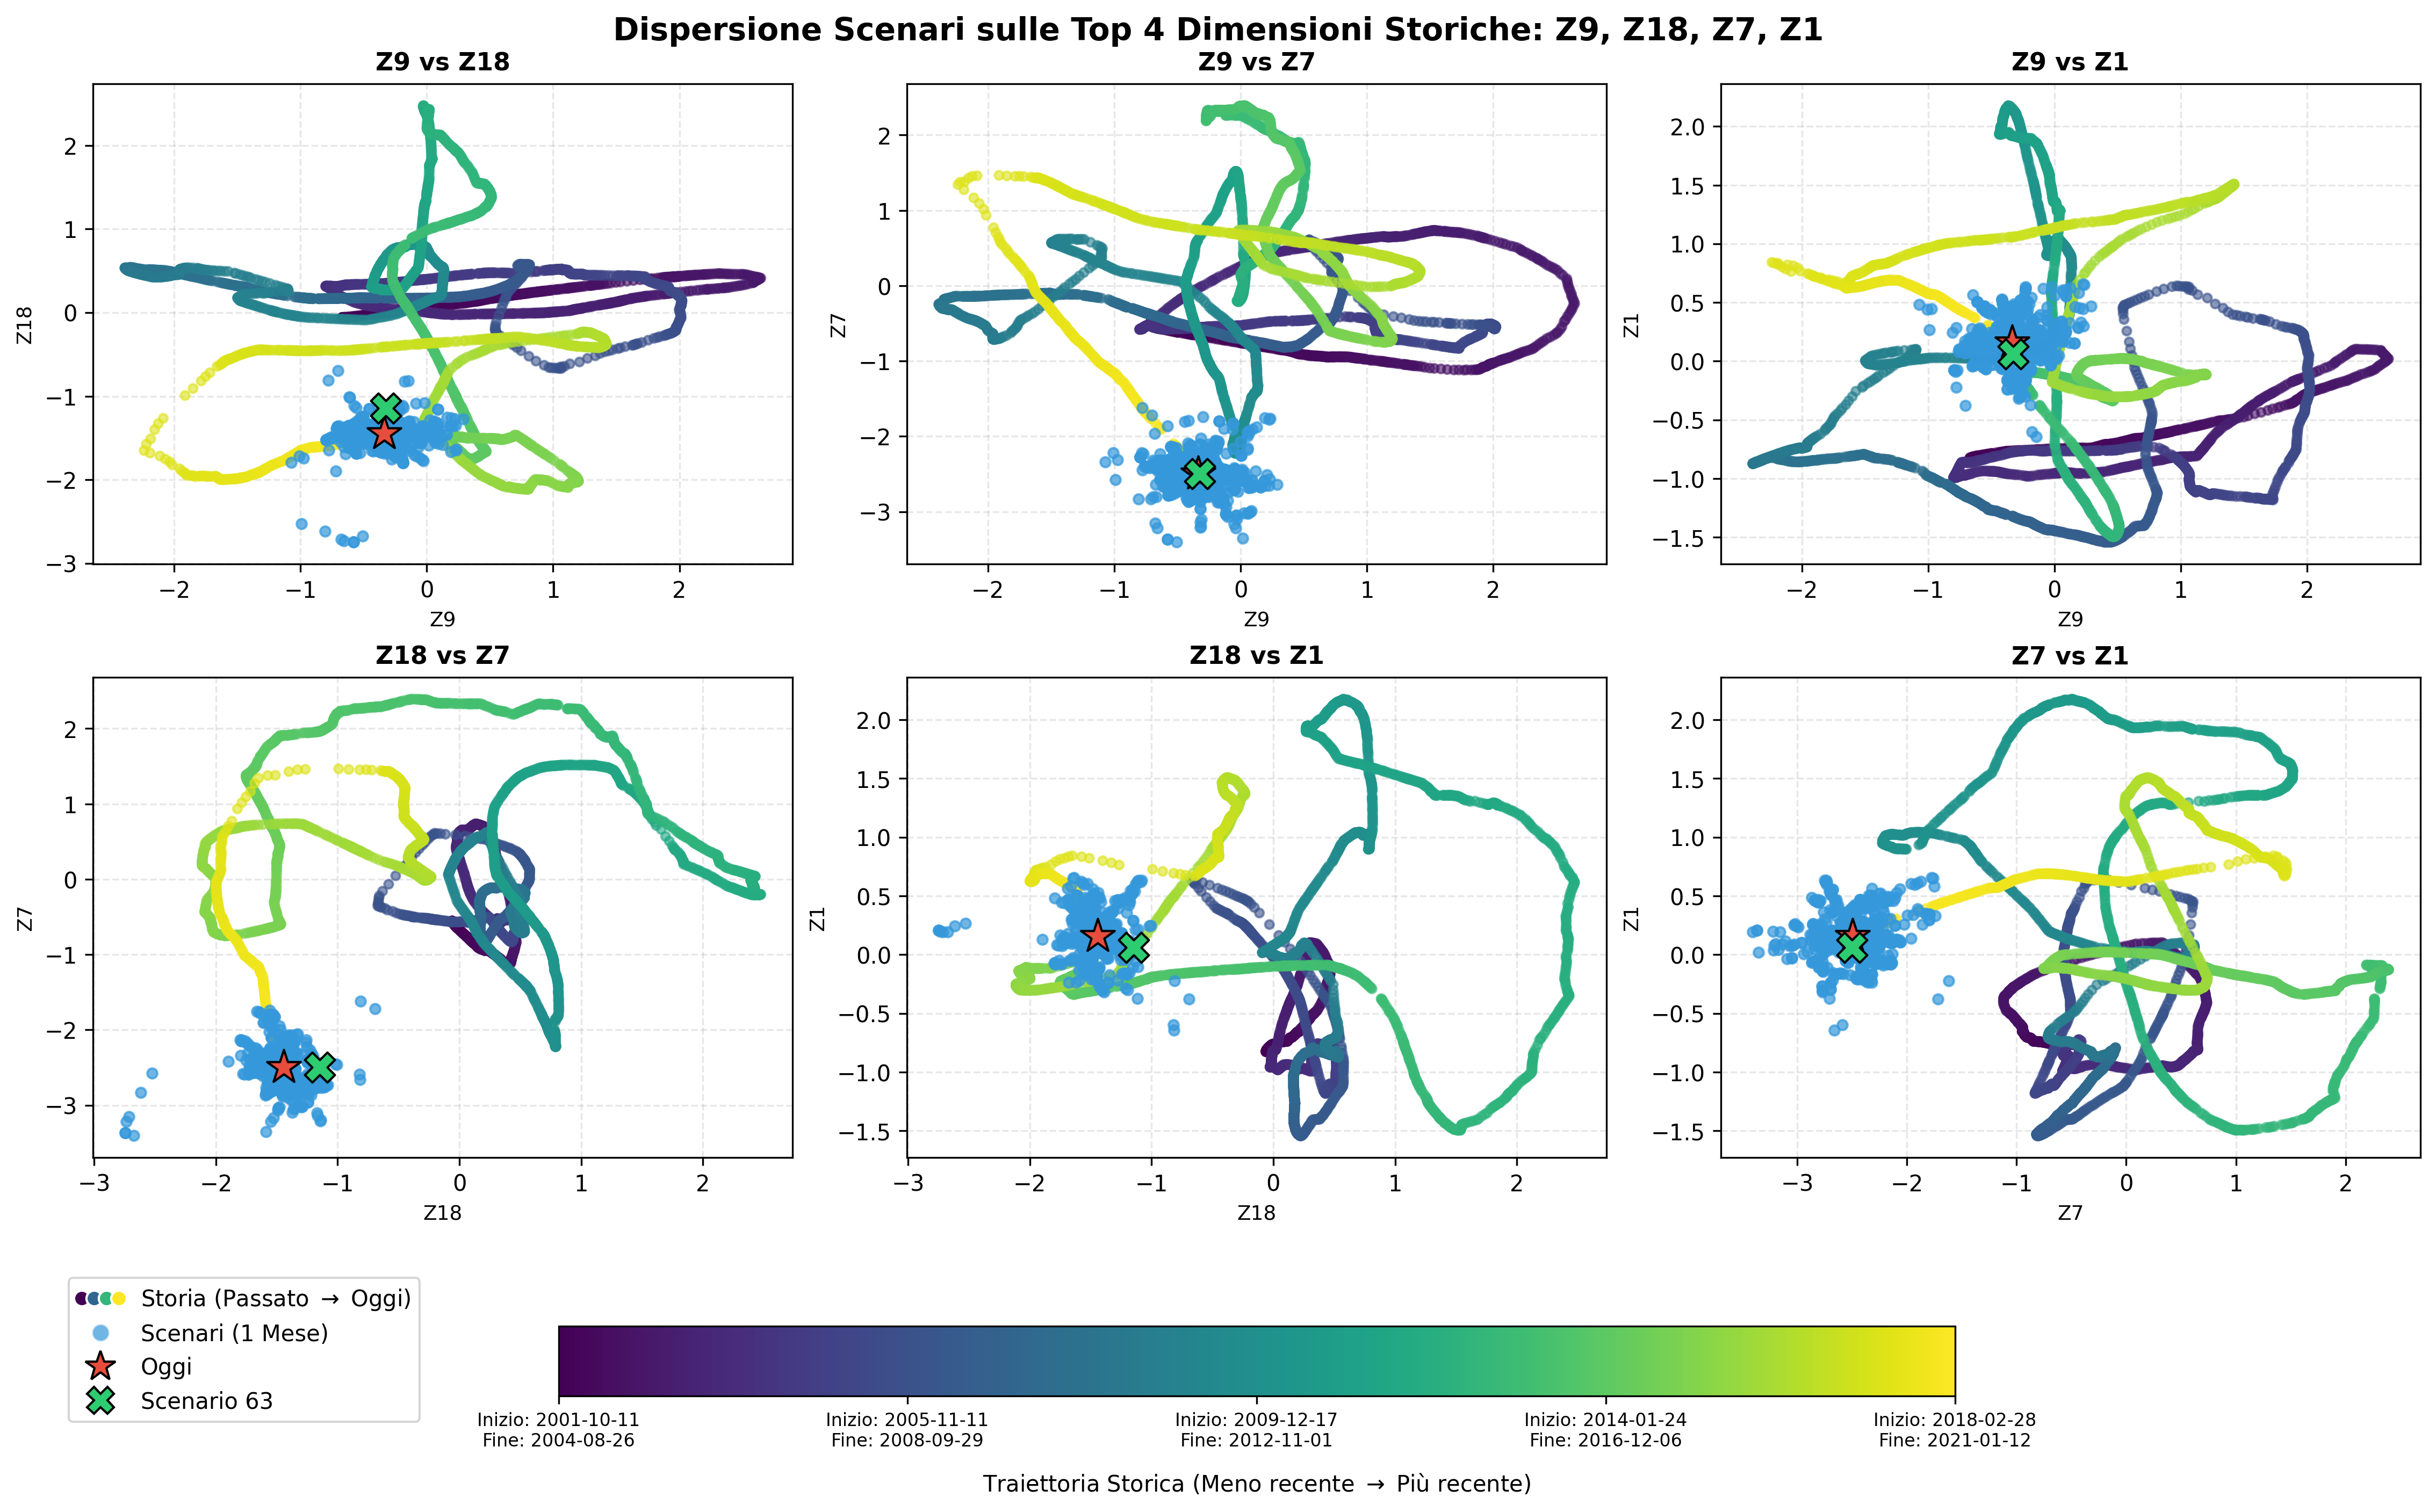
\includegraphics[width=0.9\linewidth]{Pictures/capitolo8/fig_latent_scenarios_scatter_2d.png}
\caption{Proiezioni a coppie sulle quattro dimensioni latenti a maggiore varianza storica ($Z_9$, $Z_{18}$, $Z_7$, $Z_1$): traiettoria storica dalle prime finestre valide (ottobre 2001) all'ultima (gennaio 2021), colore proporzionale al tempo, nuvola dei 1000 scenari a 21 giorni (punti azzurri), stato odierno (stella) e scenario 63 (croce).}
\label{fig:scenari}
\end{figure}

\paragraph{Verifica aggregata sui 1000 scenari (\S8.2.1).}
Ogni scenario è confrontato con la matrice odierna sui cinque fatti stilizzati del cap.~3, tradotti in indicatori scalari: la media dei coefficienti fuori diagonale; l'autovalore di mercato $\lambda_1$ e il numero di autovalori oltre il limite $\lambda_+ = 2.914$ del bulk di Marchenko-Pastur; la componente minima $\min_i v_{1,i}$ del market mode (normalizzato a somma positiva), la cui positività equivale alla proprietà di Perron-Frobenius; il rapporto $R$ fra correlazione media intra-settore e inter-settore GICS, pari a 1 in assenza di struttura settoriale (1.278 sulla matrice odierna); l'esponente $\gamma$ della distribuzione di grado dell'MST. La Tabella~\ref{tab:fatti} riporta i criteri di conformità e i due riferimenti: la matrice odierna e l'intervallo osservato sulle 412 matrici reali del bacino epurato, adottato dove la letteratura non fissa soglie assolute.

Tutti i 1000 scenari soddisfano simultaneamente i cinque fatti; tutte le matrici risultano inoltre definite positive (autovalore minimo fra 0.0101 e 0.0185), in linea con la semidefinita positività garantita per costruzione. I 65.3 milioni di coefficienti aggregati hanno media 0.4628 contro 0.4512 della matrice odierna; $\lambda_1$ resta circa due ordini di grandezza oltre $\lambda_+$; $\gamma$ cade sempre in $(2, 3)$, mentre solo il 64.1\% delle 412 matrici reali vi ricade. La tesi ne propone una spiegazione topologica plausibile: nelle finestre storiche con un hub dominante il grado massimo dell'MST arriva a 36 e la pendenza log-log si appiattisce, mentre negli scenari il grado massimo resta fra 12 e 18.

\begin{table}[htbp]
\centering
\small
\begin{tabular}{@{}llcccc@{}}
\toprule
Fatto stilizzato & Criterio & Scenari (1000) & Odierna & Reali (412) & Conformi \\
\midrule
FS1 Distribuzione & spostamento & [0.4609, 0.5352] & 0.4512 & [0.2240, 0.5070] & 1000/1000 \\
\quad (media pairwise) & \quad positivo & & & & \\
\addlinespace
FS2 Marchenko-Pastur & $\lambda_1 \gg \lambda_+$ & [172.4, 197.2] & 169.1 & [85.4, 186.8] & 1000/1000 \\
\quad ($\lambda_1$; modi $> \lambda_+$) & \quad almeno 2 modi & [7, 9] & 9 & [7, 12] & \\
\addlinespace
FS3 Perron-Frobenius & $> 0$ & [0.0164, 0.0227] & 0.0151 & [0.0007, 0.0288] & 1000/1000 \\
\quad ($\min_i v_{1,i}$) & & & & & \\
\addlinespace
FS4 Gerarchia & $> 1$ & [1.198, 1.268] & 1.278 & [1.165, 1.814] & 1000/1000 \\
\quad ($R$ intra/inter) & & & & & \\
\addlinespace
FS5 MST scale-free & $2 < \gamma < 3$ & [2.053, 2.306] & 2.119 & [1.676, 2.340] & 1000/1000 \\
\quad (esponente $\gamma$) & & & & & \\
\midrule
\multicolumn{5}{@{}l}{Tutti e cinque i fatti stilizzati simultaneamente} & 1000/1000 \\
\bottomrule
\end{tabular}
\caption{Verifica aggregata dei cinque fatti stilizzati sui 1000 scenari generati dal modello \texttt{VAE\_20dim\_cholesky\_06\_loss} (Tabella 8.1 della tesi): intervallo [min, max] sugli scenari, valore della matrice odierna (finestra chiusa il 12 gennaio 2021) e intervallo [min, max] sulle 412 matrici reali del bacino epurato.}
\label{tab:fatti}
\end{table}

\begin{riquadro}{Osservazione: lo scenario 311}
La correlazione media dello scenario 311 (0.5352) supera lievemente l'estremo superiore dell'intervallo tipico $[0.2, 0.5]$ del cap.~3. Non è una violazione: il fatto stilizzato prescrive uno spostamento sistematico verso valori positivi, che uno scenario più correlato soddisfa a maggior ragione, e l'intervallo descrive la magnitudo dei regimi ordinari, non un limite algebrico. Scenari così sincronizzati, tipici delle fasi di stress, sono in ottica di rischiosità la porzione più interessante della distribuzione.
\end{riquadro}

\paragraph{Ispezione dello scenario 63 (\S8.2.2).}
A complemento degli indicatori scalari, la tesi ripercorre graficamente i cinque fatti sullo scenario 63, scelto a fini espositivi. Media e mediana pairwise valgono 0.4635 e 0.4711 contro 0.4512 e 0.4593 della matrice odierna; $\lambda_1$ vale 173.2 contro 169.1, con nove autovalori oltre il bulk in entrambe. Il market mode ha componenti tutte dello stesso segno e similarità coseno 0.9999 con quello odierno (0.9893 e 0.9883 per il secondo e il terzo autovettore); il dendrogramma ripropone gli stessi blocchi settoriali GICS; l'esponente scale-free è 2.227 contro 2.119, con grado massimo 14 contro 15.

%% ---- sezione F: conclusioni ----
\section{Conclusioni, limiti e sviluppi futuri}

La sintesi dei risultati (cap.~9, \S9.1) si può condensare in quattro punti.
\begin{itemize}[nosep]
\item Il primo tentativo sulla matrice di correlazione grezza non rispettava in modo affidabile la semidefinita positività (PSD); da qui il passaggio definitivo al fattore di Cholesky, con matrice ricomposta come $L L^{\top}$ e PSD garantita per costruzione.
\item PCA e autoencoder lineare (AE lineare) convergono, a parità di $K$, allo stesso errore, coerentemente con il teorema di Bourlard e Kamp (1988), e fissano il benchmark lineare.
\item L'autoencoder profondo (AE) supera nettamente tale limite a ogni $K$, senza segni di overfitting; il VAE (\texttt{VAE\_20dim\_cholesky\_06\_loss}) è intermedio: meno accurato dell'AE, migliore di PCA e AE lineare a $K = 20$.
\item Il valore distintivo del VAE è generativo: il block-bootstrap degli incrementi latenti produce, dallo stato di mercato osservato, una distribuzione di scenari sintetici a orizzonte nominale di 21 giorni, non come previsione puntuale ma come stima della possibile variabilità delle correlazioni a quell'orizzonte, in ottica di rischiosità. I 1000 scenari non mostrano violazioni dei cinque fatti stilizzati. L'AE deterministico non è stato impiegato per generare. Senza regolarizzazione variazionale il suo spazio latente non è vincolato ad alcuna distribuzione a priori e non ha la continuità e la densità necessarie a un campionamento significativo, che il suo obiettivo di addestramento non prevede (premessa metodologica non verificata empiricamente, \S4.3).
\end{itemize}

\paragraph{Rispetto al lavoro di riferimento.} Caprioli et al.\ (2024) addestrano un VAE con spazio latente bidimensionale su 206 matrici mensili di 44 indici (finestre di 100 mesi, 1997--2022, split 70\%/30\%) e stimano per bootstrap latente la distribuzione del Value at Risk di un portafoglio creditizio. Qui il paniere conta 362 titoli a frequenza giornaliera e ogni matrice 65\,703 coefficienti contro 946. Si aggiungono il sanity check sul benchmark lineare, l'architettura a imbuto e la loss di Jeffreys, la PSD incorporata nella rappresentazione, otto metriche di errore, l'analisi della dimensionalità effettiva, la classificazione GICS via LLM, la verifica quantitativa dei 1000 scenari e il block-bootstrap giornaliero. Restano fuori perimetro le misure di rischio di portafoglio e l'interpretazione economica delle coordinate latenti.

\paragraph{Limiti (\S9.2).} Il capitolo ne dichiara sei.
\begin{itemize}[nosep]
\item Survivorship bias, il limite più forte perché agisce a monte: i risultati si riferiscono al ``mercato dei titoli sopravvissuti'' e gli scenari possono risultare conservativi nelle crisi.
\item Verifica aggregata ridotta a indicatori scalari, ispezione visiva di un solo scenario, numerosità effettiva sotto 1000 per i blocchi sovrapposti, un solo stato iniziale.
\item Sovrapposizione fra finestre fino al 98.6\% e assenza di separazione temporale fra i set: possibile ottimismo nelle metriche.
\item VAE non testato a $K = 3$ e $K = 100$; errore che non decresce con $K$ (MSE da $1.26$ a $1.88 \times 10^{-4}$ fra $K = 10$ e $K = 30$), coerentemente con il posterior collapse.
\item Perimetro ristretto al regime cooperativo (49 finestre escluse).
\item Classificazione GICS via LLM non sottoposta a validazione incrociata con fonti ufficiali.
\end{itemize}

\paragraph{Sviluppi futuri (\S9.3).} Le direzioni sono cinque.
\begin{itemize}[nosep]
\item Applicazione degli scenari al rischio di portafogli reali.
\item Verifica da più stati iniziali e test formali di aderenza distributiva.
\item Confronto con CorrGAN (Marti, 2020) e modelli di diffusione.
\item Rimozione del survivorship bias con un panel a composizione variabile.
\item Altre asset class (valute, materie prime) e purging esplicito fra i set.
\end{itemize}


\end{document}
